\section{Simulazioni modello di Ising 1D}

Prima di iniziare lo studio computazionale del modello, è stati determinati i parametri simulativi ottimali. In questa fase ho 
considerato catene di spin di lunghezza 

$$
N \in \left\{1000,\,3000,\,6000,\,10000\right\}
$$

alle temperature

$$
T \in \left\{0.5,\,1.0,\,1.5,\,2.0\right\}
$$

in condizione di presenza ed assenza di campo magnetico. I risultati ottenuti in questa fase sono riportati in modo rissuntivo 
nella seguente figura, comprensiva di entrambe le casistiche. 

\begin{figure}[H]
    \centering
    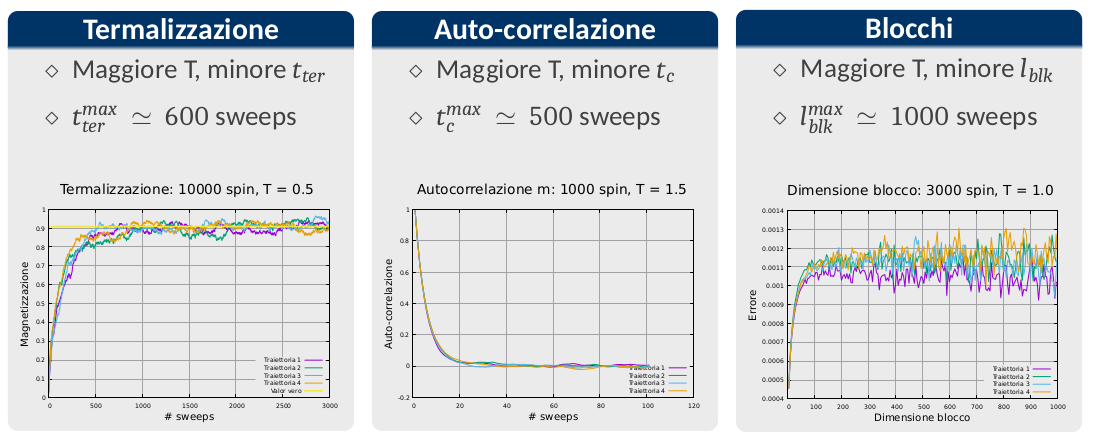
\includegraphics[width=\textwidth]{Immagini/simIsing1D/carMetro.png}
    \caption{Caratterizzazione metodo di Metropolis}
    \label{fig: car_Ising1D}
\end{figure}



\subsection{Osservabili}


\begin{figure}[htbp]
    \centering
    \begin{minipage}{0.5\textwidth}  
      \centering
      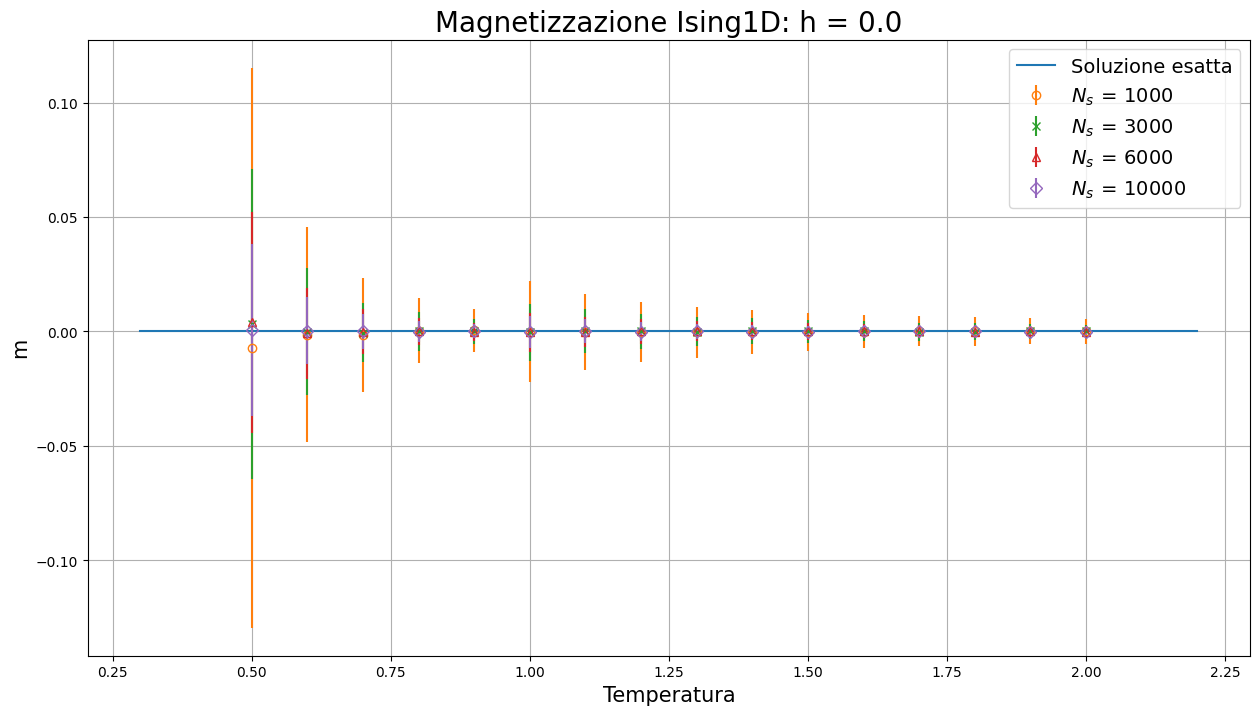
\includegraphics[page=1, width=\textwidth]{Immagini/simIsing1D/magn_h0.0.png}
      \caption{Magnetizzazione: h = 0.0.}
    \end{minipage}\hfill
    \begin{minipage}{0.5\textwidth}  
      \centering
      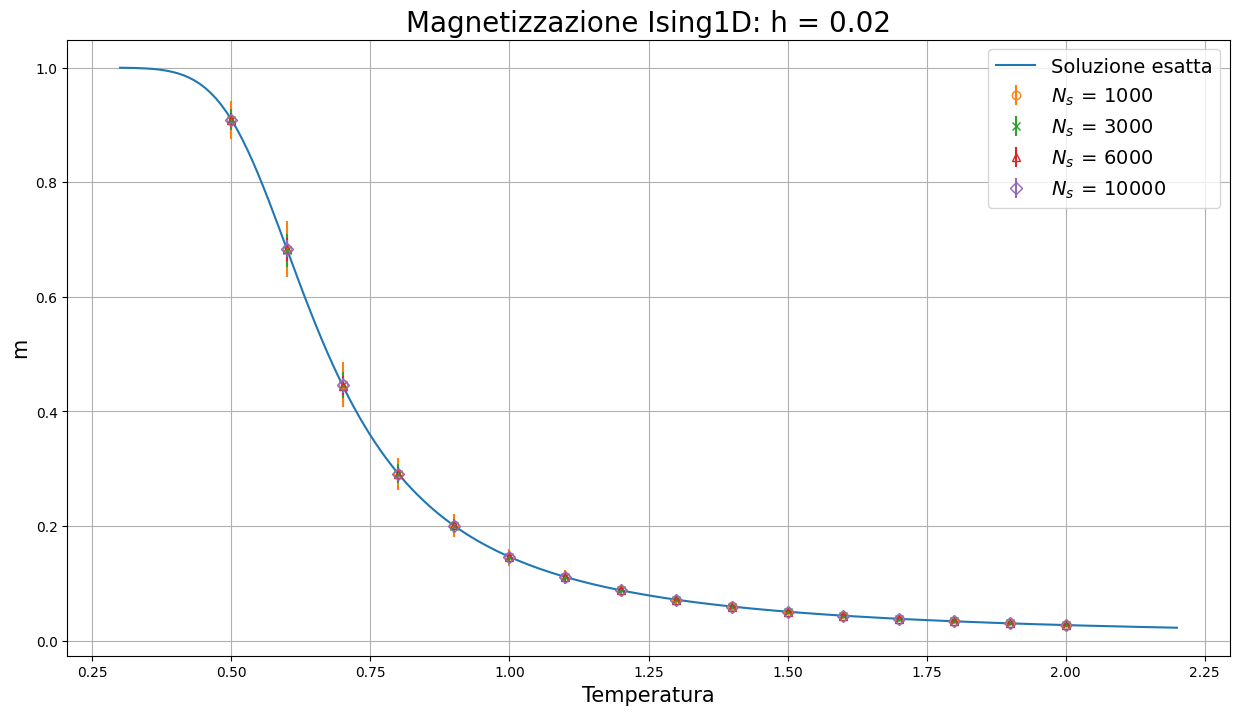
\includegraphics[page=1, width=\textwidth]{Immagini/simIsing1D/magn_h0.02.png}
      \caption{Magnetizzazione: h = 0.02.}
    \end{minipage}
\end{figure}

\begin{figure}[H]
    \centering
    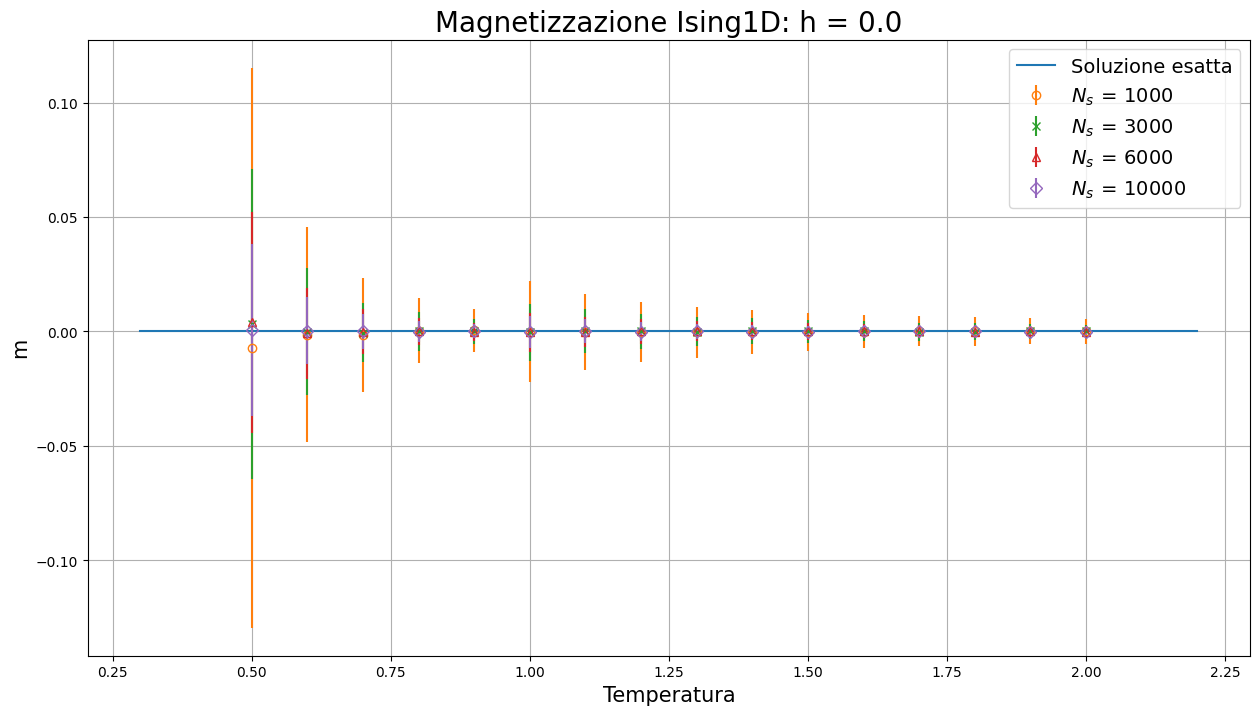
\includegraphics[width=\textwidth]{Immagini/simIsing1D/magn_h0.0.png}
    \caption{Magnetizzazione modello di Ising 1D: h = 0.0.}
    \label{fig: magn_Ising1D_h0.0}
\end{figure}

\begin{figure}[H]
    \centering
    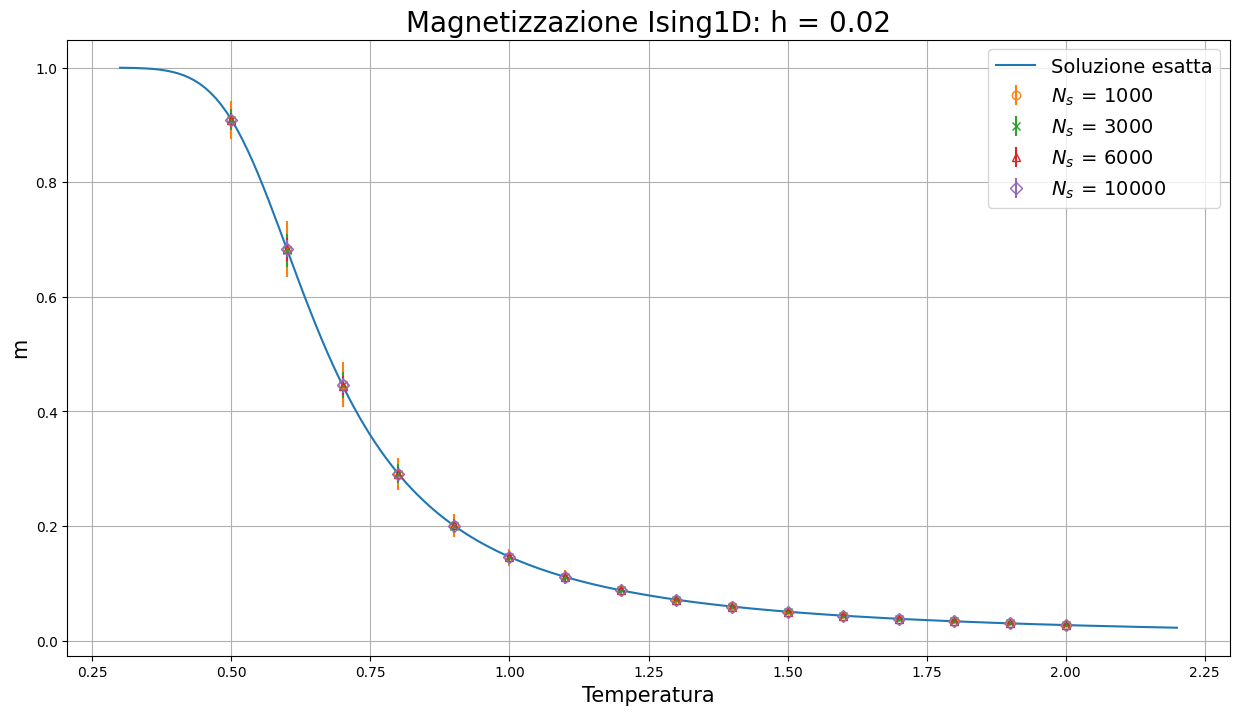
\includegraphics[width=\textwidth]{Immagini/simIsing1D/magn_h0.02.png}
    \caption{Magnetizzazione modello di Ising 1D: h = 0.02.}
    \label{fig: magn_Ising1D_h0.02}
\end{figure}

\begin{figure}[H]
    \centering
    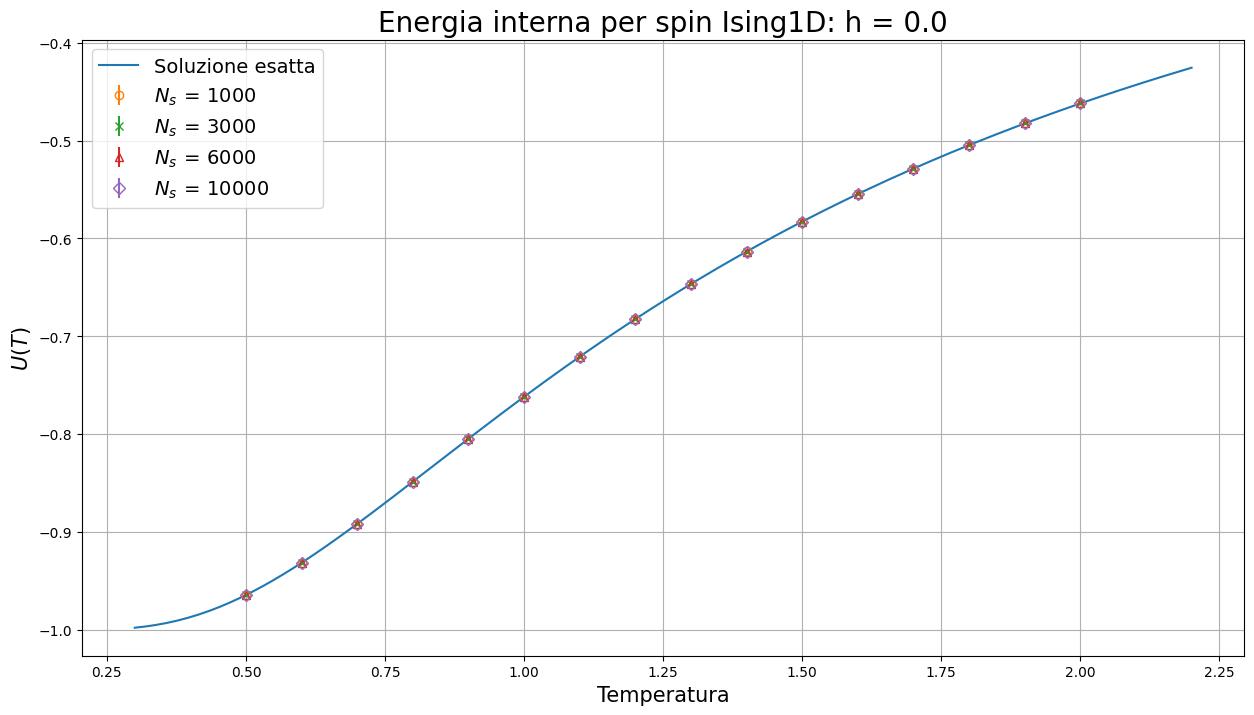
\includegraphics[width=\textwidth]{Immagini/simIsing1D/ene_h0.0.png}
    \caption{Energia modello di Ising 1D: h = 0.0.}
    \label{fig: ene_Ising1D_h0.0}
\end{figure}

\begin{figure}[H]
    \centering
    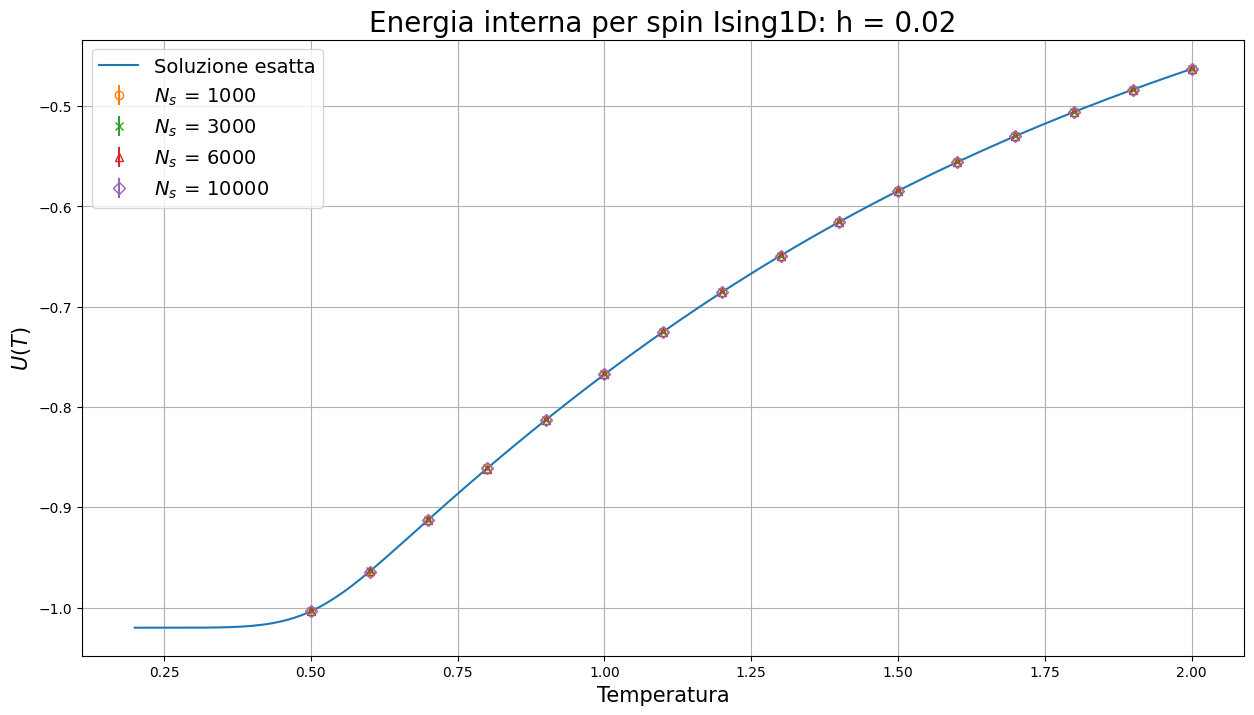
\includegraphics[width=\textwidth]{Immagini/simIsing1D/ene_h0.02.png}
    \caption{Energia modello di Ising 1D: h = 0.02.}
    \label{fig: ene_Ising1D_h0.02}
\end{figure}

\begin{figure}[H]
    \centering
    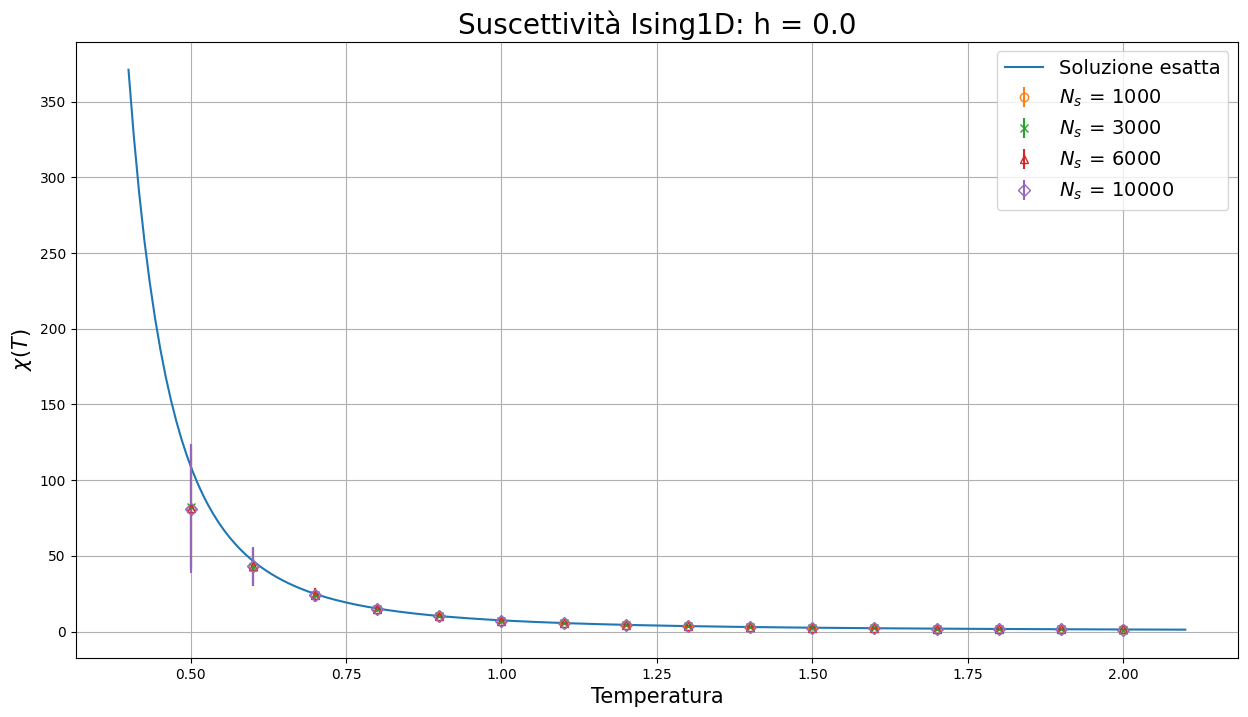
\includegraphics[width=\textwidth]{Immagini/simIsing1D/chi_h0.0.png}
    \caption{Suscettività modello di Ising 1D: h = 0.0.}
    \label{fig: chi_Ising1D_h0.0}
\end{figure}

\begin{figure}[H]
    \centering
    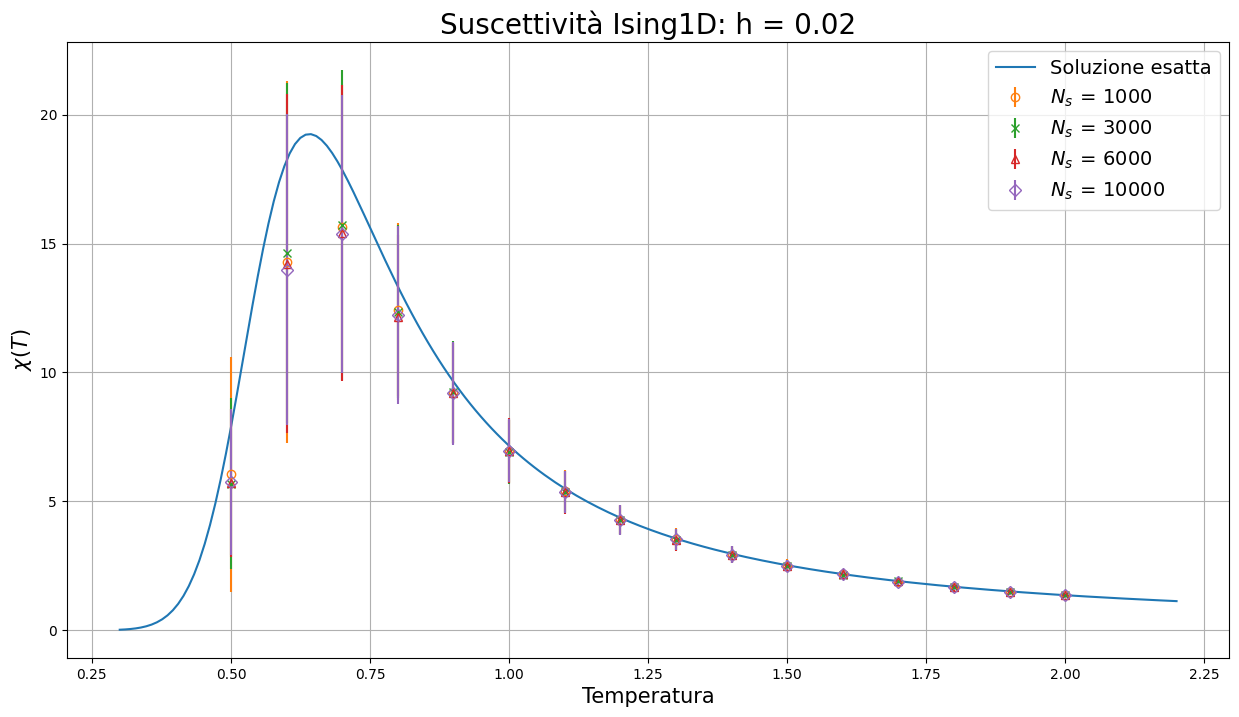
\includegraphics[width=\textwidth]{Immagini/simIsing1D/chi_h0.02.png}
    \caption{Suscettività modello di Ising 1D: h = 0.02.}
    \label{fig: chi_Ising1D_h0.0}
\end{figure}

\begin{figure}[H]
    \centering
    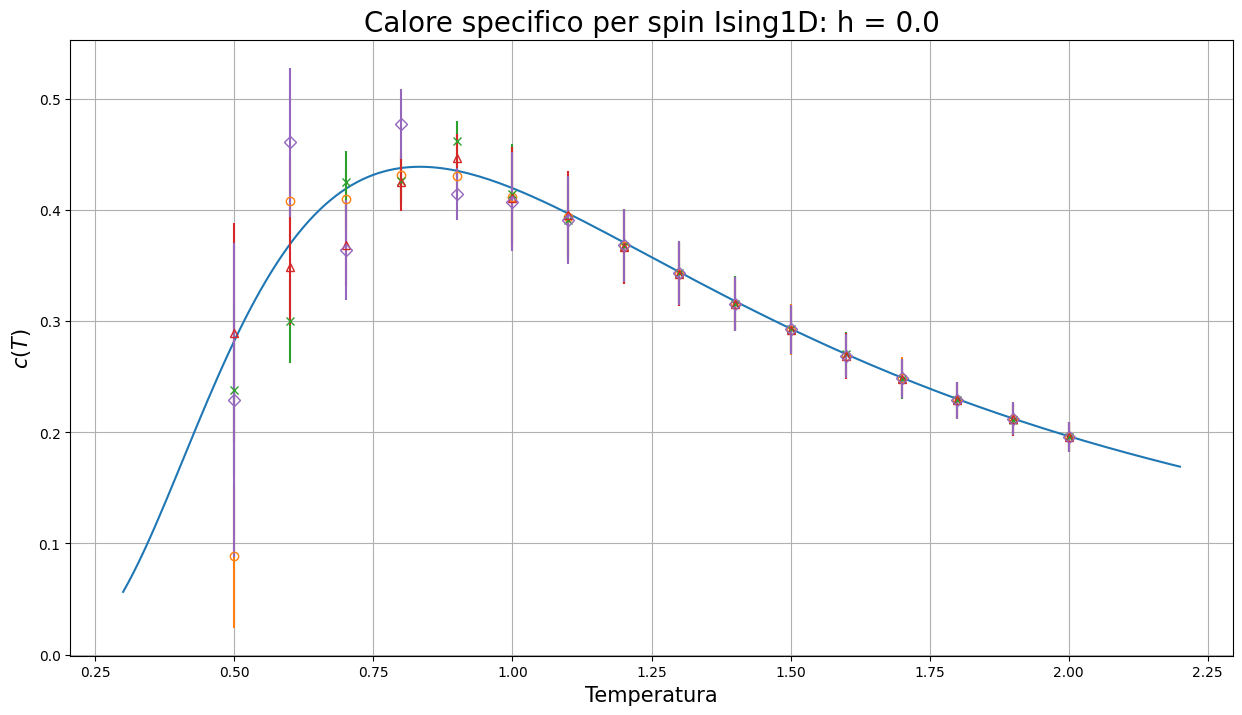
\includegraphics[width=\textwidth]{Immagini/simIsing1D/cp_h0.0.png}
    \caption{Calore specifico modello di Ising 1D: h = 0.0.}
    \label{fig: cp_Ising1D_h0.0}
\end{figure}

\begin{figure}[H]
    \centering
    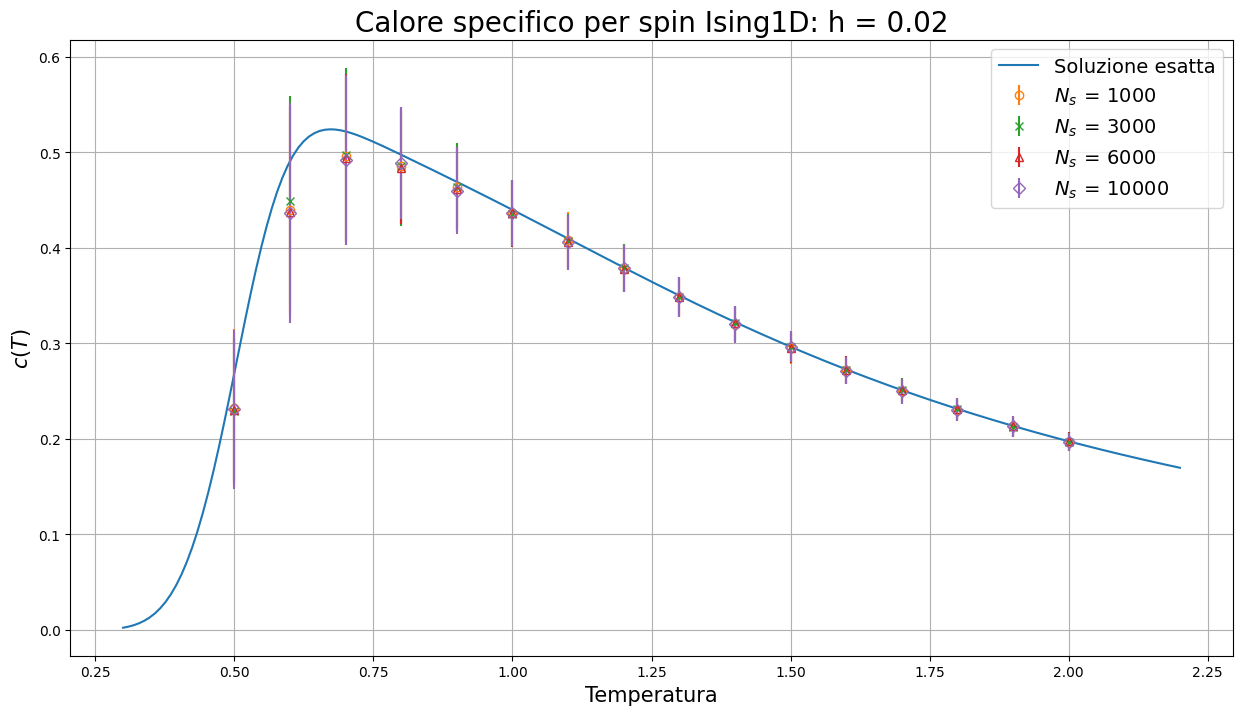
\includegraphics[width=\textwidth]{Immagini/simIsing1D/cp_h0.02.png}
    \caption{Calore specifico modello di Ising 1D: h = 0.02.}
    \label{fig: cp_Ising1D_h0.0}
\end{figure}